\section{Glyph-based Solutions for Biological Sequence Analysis}
\label{sec:sequence_logo}

%-------------------------------------------------------------------------
Advances in DNA sequencing technologies have turned a time consuming and expensive process into a quasi-mainstream commodity.
Next generation sequencing allows exploration of the blueprints of life in fascinating new ways, making the genome of thousands of species available to computational analysis.
Of particular interest to scientists is the detection of regions of genomes under selective pressure and to ascertain which regions of DNA, RNA and proteins are functionally and/or structurally important across species (\eg, the conserved regions of a protein in mice, human, rat, and horse).

Although our ability to process this data has increased, the methods used to visualize and report this conservation in scientific publications has not moved on in over 20 years.
This dominant method, named the ``sequence logo'' \cite{Schneider.Stephens1990,Schneider2002} is comprised of a series of letters stacked on top of each other.
It is reliance on these letters and their arrangement that cause perception problems \cite{biovis_redesign}. 
%
Here we introduce a new sequence logo design aimed at addressing their perception issues using design principles from Chapter \ref{chap:related_work}. 
Our approach is a three stage process, with a domain-expert always in the loop:

\begin{enumerate}
\item improving the current \emph{sequence logo} design to address perceptual issues caused by: a) use of letter size to represent value; and b) the arrangement of letters on the y-axis, which can make residues look more conserved than others based on the number of letters it is stacked upon;

\item adding \emph{glyphs} to annotate positions with chemical properties of particular residues to aid interpretation of the effect of alternations in different species for example; and

\item an evaluation of the redesigned sequence logo with both advanced and 'naive' sequence logo users to ascertain the benefits of the new design.
\end{enumerate}

\subsection{Background}

Transcription factors, as shown in Figures \ref{fig:binding} A and B are proteins with a central function; they can, with high specificity, recognize and bind to DNA regions, triggering transcription of DNA into RNA.
These DNA regions are known as transcription factor binding sites (TFBS) and their identification is essential to the reconstruction of transcriptional regulatory networks of cells.
As shown in Figure \ref{fig:binding} C, sequence comparison across organisms can be used to highlight areas of conservation to pinpoint unknown TFBS.
Low variability at some position $i$ generally points to a level of functional importance in that region of DNA or protein, pointing to selective pressure. 

\begin{figure}[h!]
\centering
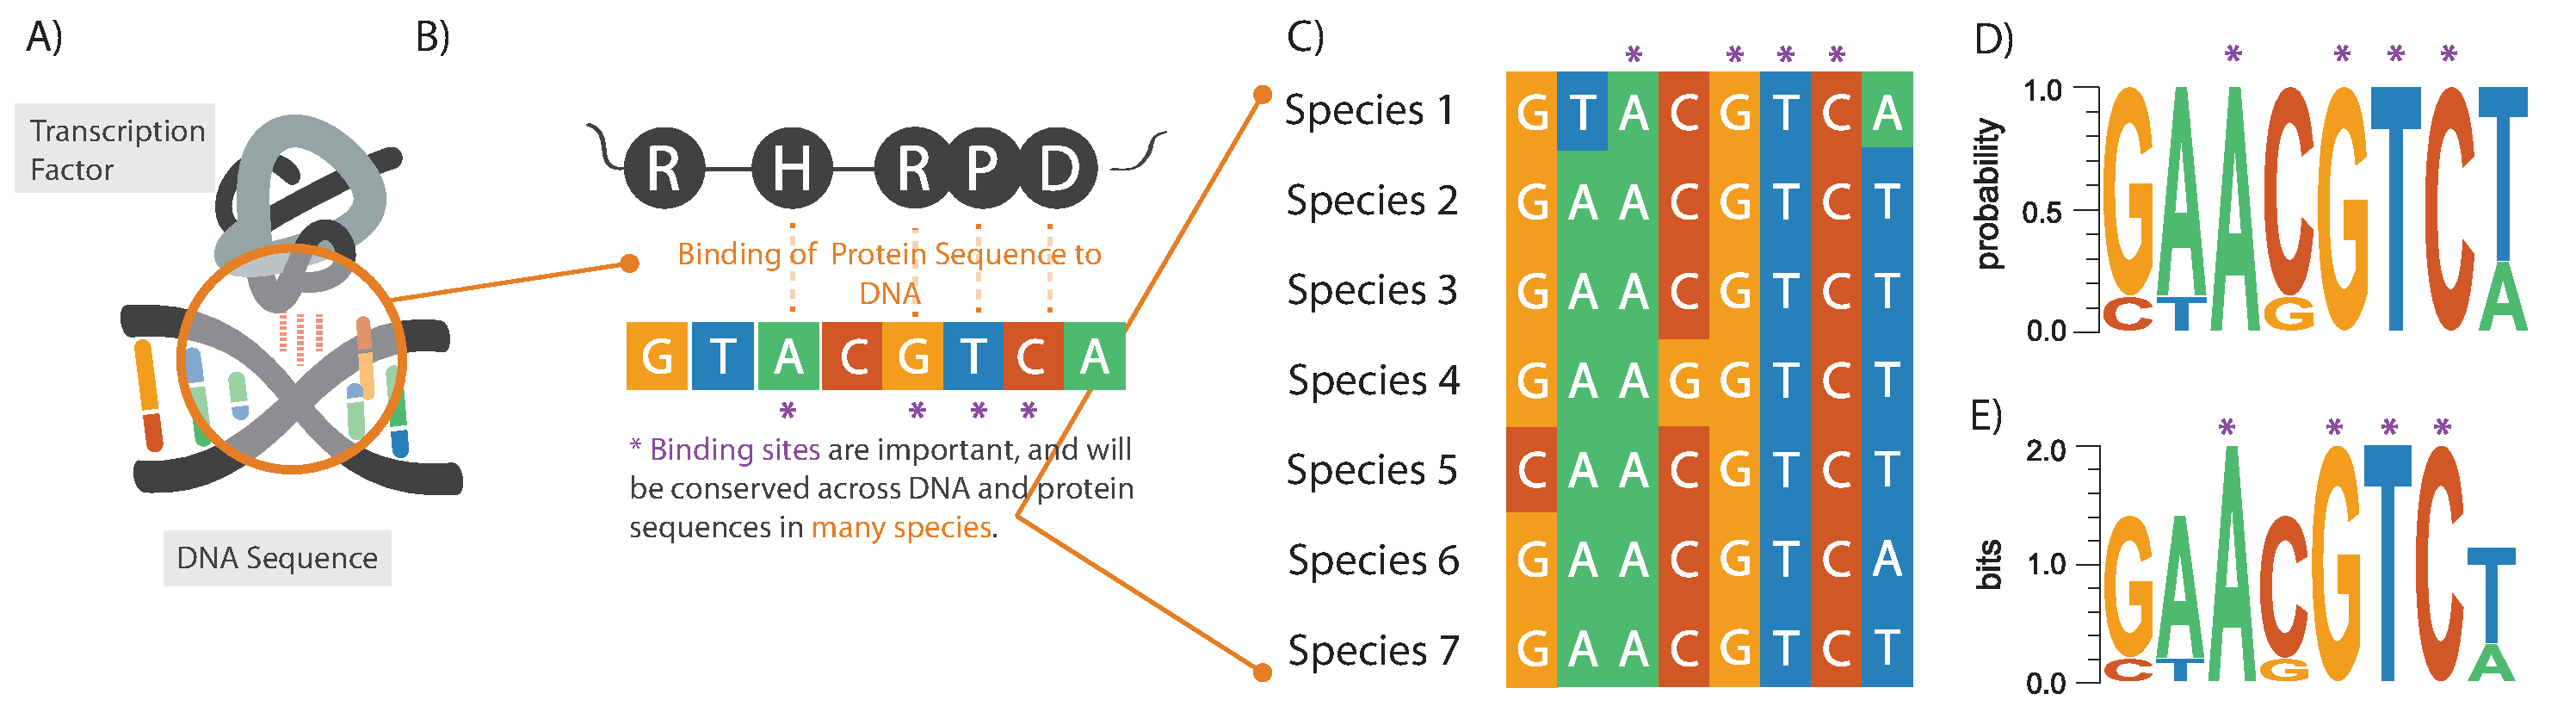
\includegraphics[width=\textwidth]{images/other_glyphs/sequence_logo/binding}
\caption{A) An abstraction of a transcription binding site where a protein binds to a region of DNA.
B) Certain residues, amino acids for the protein and DNA nucleotides for DNA are important in creating a bond between the DNA and protein to enable some function to occur (\eg, DNA repair).
C) The DNA of seven species is compared which shows a number of conserved regions where the DNA nucleotide is always the same (marked with a blue asterix). In a large matrix with many hundreds or thousands of sequences, this can be difficult to visualize.
D) Sequence logos provide a way of showing conserved regions. Probability based sequence logos assign the height of a letter in proportion to the number of times it appeared in that position.
E) Entropy-based sequence logos adjust the height of each letter based on the amount of ``surprise'' at each sequence rather than just the probability.}
\label{fig:binding}
\end{figure}

In order to visualize these binding sites, sequence logos were devised as a visualization technique to view a position weight matrix (PWM), which specifies for each position in a sequence the likelihood of observing a particular residue (DNA/RNA nucleotide or amino acid). From this matrix, a simple frequency-based sequence logo can be drawn by iterating through each position $i$ in the sequence (see Figure \ref{fig:binding} D). For each position, the height of each letter $a$ can be calculated as $p(a) \times R$ where $p(a)$ is the measured probability of $a$ occurring at position $i$, and $R$ is the maximum height at position $i$.

An alternative approach is to determine the maximum height at position $i$ by computing its ``information content'', a term derived from Claude Shannon's information theory\cite{Shannon1948}.
Information content represents the level of certainty at a specific position $i$ by measuring how much the probability distribution of the detected letters in that position deviates from a uniform distribution, where all valid letters have an equiprobable chance of occurring.
Given $s$ valid letters, $a_j, j=1, 2, \ldots, s$, in an alphabet $\mathbb{Z}$ and their probability distribution function, $p(a_j)$, the level of uncertainty can be defined by the following entropy measure:
\[
H(\mathbb{Z}) = -\sum_{j=1}^s p(a_j) log_2 p(a_j)
\]

\noindent where the logarithm is base two, and the unit for the uncertainty $H$ is ``bit''.
For an equiprobable distribution, $p(a_j) = 1/s$ for all letters in the alphabet $\mathbb{Z}$.
The above entropy measure yields the maximum uncertainty (commonly referred to as the maximum entropy), $H_{max}(s) = log_2 (s)$.

\noindent For example, for twenty-one amino acids, we have $H_{max}(21) = 4.39$ bits, and for 4 types of nucleic acids, $H_{max}(4) = 2$ bits.

Since it is unlikely that there is an equiprobable distribution of letters at each position $i$, the actual uncertainty is usually less than $H_{max}$.
Therefore the difference between the maximum uncertainty and the measured uncertainty can be defined as the certainty, which is visually encoded as the total height $R_i$ for all letters at position $i$.

As shown in Figure \ref{fig:binding} E, a high stack indicates a high level of certainty with a strong preference for one or at most two nucleotides.
A low stack implies a low level of certainty with many possibilities.
The idea behind this visual design is that the highly conserved positions ``pop out'' more due to their greater height.

%\subsection{Related Work}
%
%There have been a few attempts to redesign the sequence logo in the past, with most having focused on modifying how such letters are positioned on the y-axis with Kullback Leibler \cite{kullback1951}, position-specific scoring matrix (PSSM) \cite{fujii2004}, and berry logos \cite{berry2006,berrylogo}. These in part can alleviate some of the perception issues with the sequence logo, though all continue to use letters to represent size apart from LogoBar by Perez \emph{et al} \cite{perez2006logobar}. We extend on the work by Perez through support for DNA/RNA sequences, glyphs, an evaluation and a web-based implementation.

%-------------------------------------------------------------------------

\subsection{Design Process}

Our design process involved the application of design principles from Chapter \ref{chap:related_work} to help in the creation of a new sequence logo that circumvented frailties in the old design.
This process involved the following steps where there were both feedforward and feedback steps:

\begin{enumerate}
\item\textbf{Review of original design with domain experts}; 
\item\textbf{Presentation of design options};
\item\textbf{Implementation}; and
\item\textbf{Evaluation using an online user survey}.
\end{enumerate}

\begin{figure}[t!]
\centering
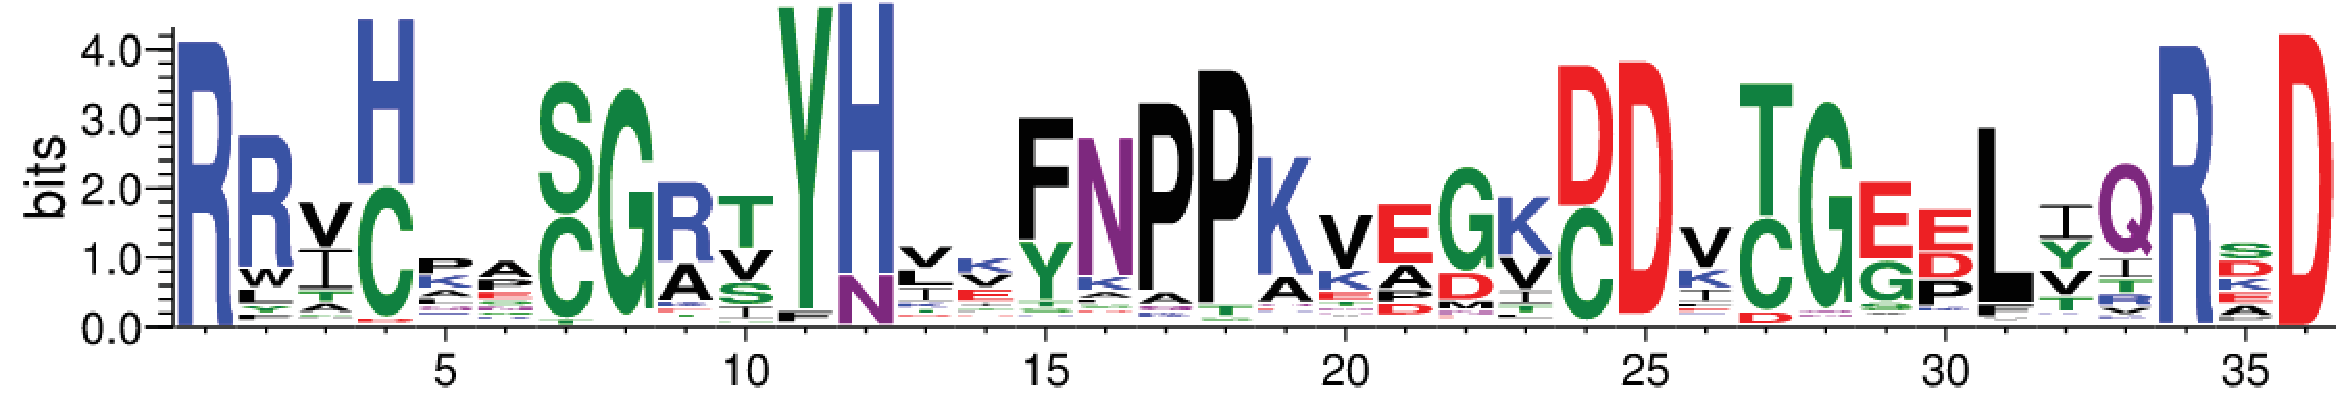
\includegraphics[width=\textwidth]{images/other_glyphs/sequence_logo/old-sequence-logo}
\caption{A traditional sequence logo generated using WebLogo \url{http://weblogo.threeplusone.com} from the BioVis redesign contest data \cite{biovis_redesign} showing the conserved regions across 1809 protein sequences.}
\label{fig:sequence_logo_design_teaser}
\end{figure}

\textbf{Review of original design with domain experts}. The weaknesses of the original sequence logo may be summarized as follows: 
\begin{enumerate}
\item \emph{Using letter size to show value} --- letters have an undesirable property in that they are of differing densities. We have quantified this effect (see Figure \ref{fig:letter-area}) and found that and \emph{R}, \emph{H} and \emph{W} take up to about three times as much ink as \emph{I} ,\emph{J} or \emph{L} for example.
When used for space filling, this ultimately leads to perception issues as denser letters will be more visible.
Use of letters also means that when there many variants at a given position, letters become ``squashed'' so it is often impossible to read them;

\begin{figure}[b!]
\centering
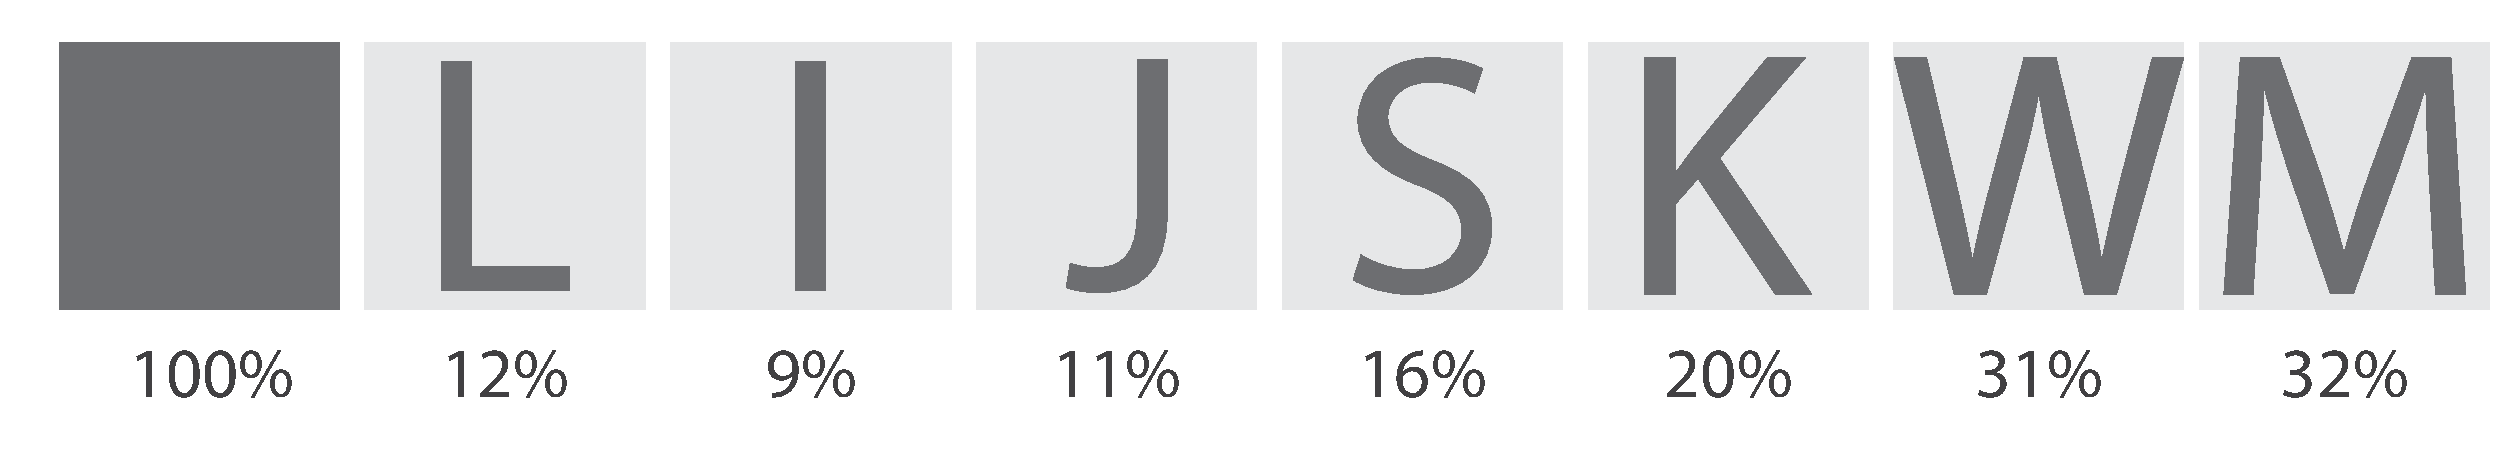
\includegraphics[width=.6\textwidth]{images/other_glyphs/sequence_logo/space}
\caption{The amount of ink used in a letter can influence the perceived `weight' of the letter. \emph{W} and \emph{M} take up three times as much ink as \emph{I}, \emph{J}, and \emph{L}, and twice as much as \emph{S}.}
\label{fig:letter-area}
\end{figure}

\item \emph{Placement of the most dominant letter on top of the less dominant letters, leading to possible misinterpretation of the size of a letter depending on where it is placed on the y axis} --- this is particularly evident in Figure \ref{fig:sequence_logo_design_teaser} at positions 2 and 4 where we may compare heights between `R' (Arginine) and `H' (Histidine).
In Figure \ref{fig:sequence_logo_design_teaser}, `H' is positioned higher in the chart due to the letters below it.
This gives the impression that the conservation of `H' at position 4 is greater than the conservation of `R' at position 2. In reality, `R' is more conserved at position 2.
\end{enumerate}

\textbf{Presentation of design options}. Any new design should retain the core principles of the original sequence logo to ease uptake of a new representation, whilst subtly overcoming its perception issues.
Initially, this design process involved the creation of a number of options shown in Figure \ref{fig:sequence_design_options} to improve on the current letter-based approach. 
These design options were filtered to just one following feedback from domain experts as well as consideration of research presented in Chapter \ref{chap:related_work}, in particular the research by Cleveland and McGill \cite{cleveland1984graphical}, and Heer and Bostock \cite{heer2010crowdsourcing}.

\begin{figure}[t!]
\centering
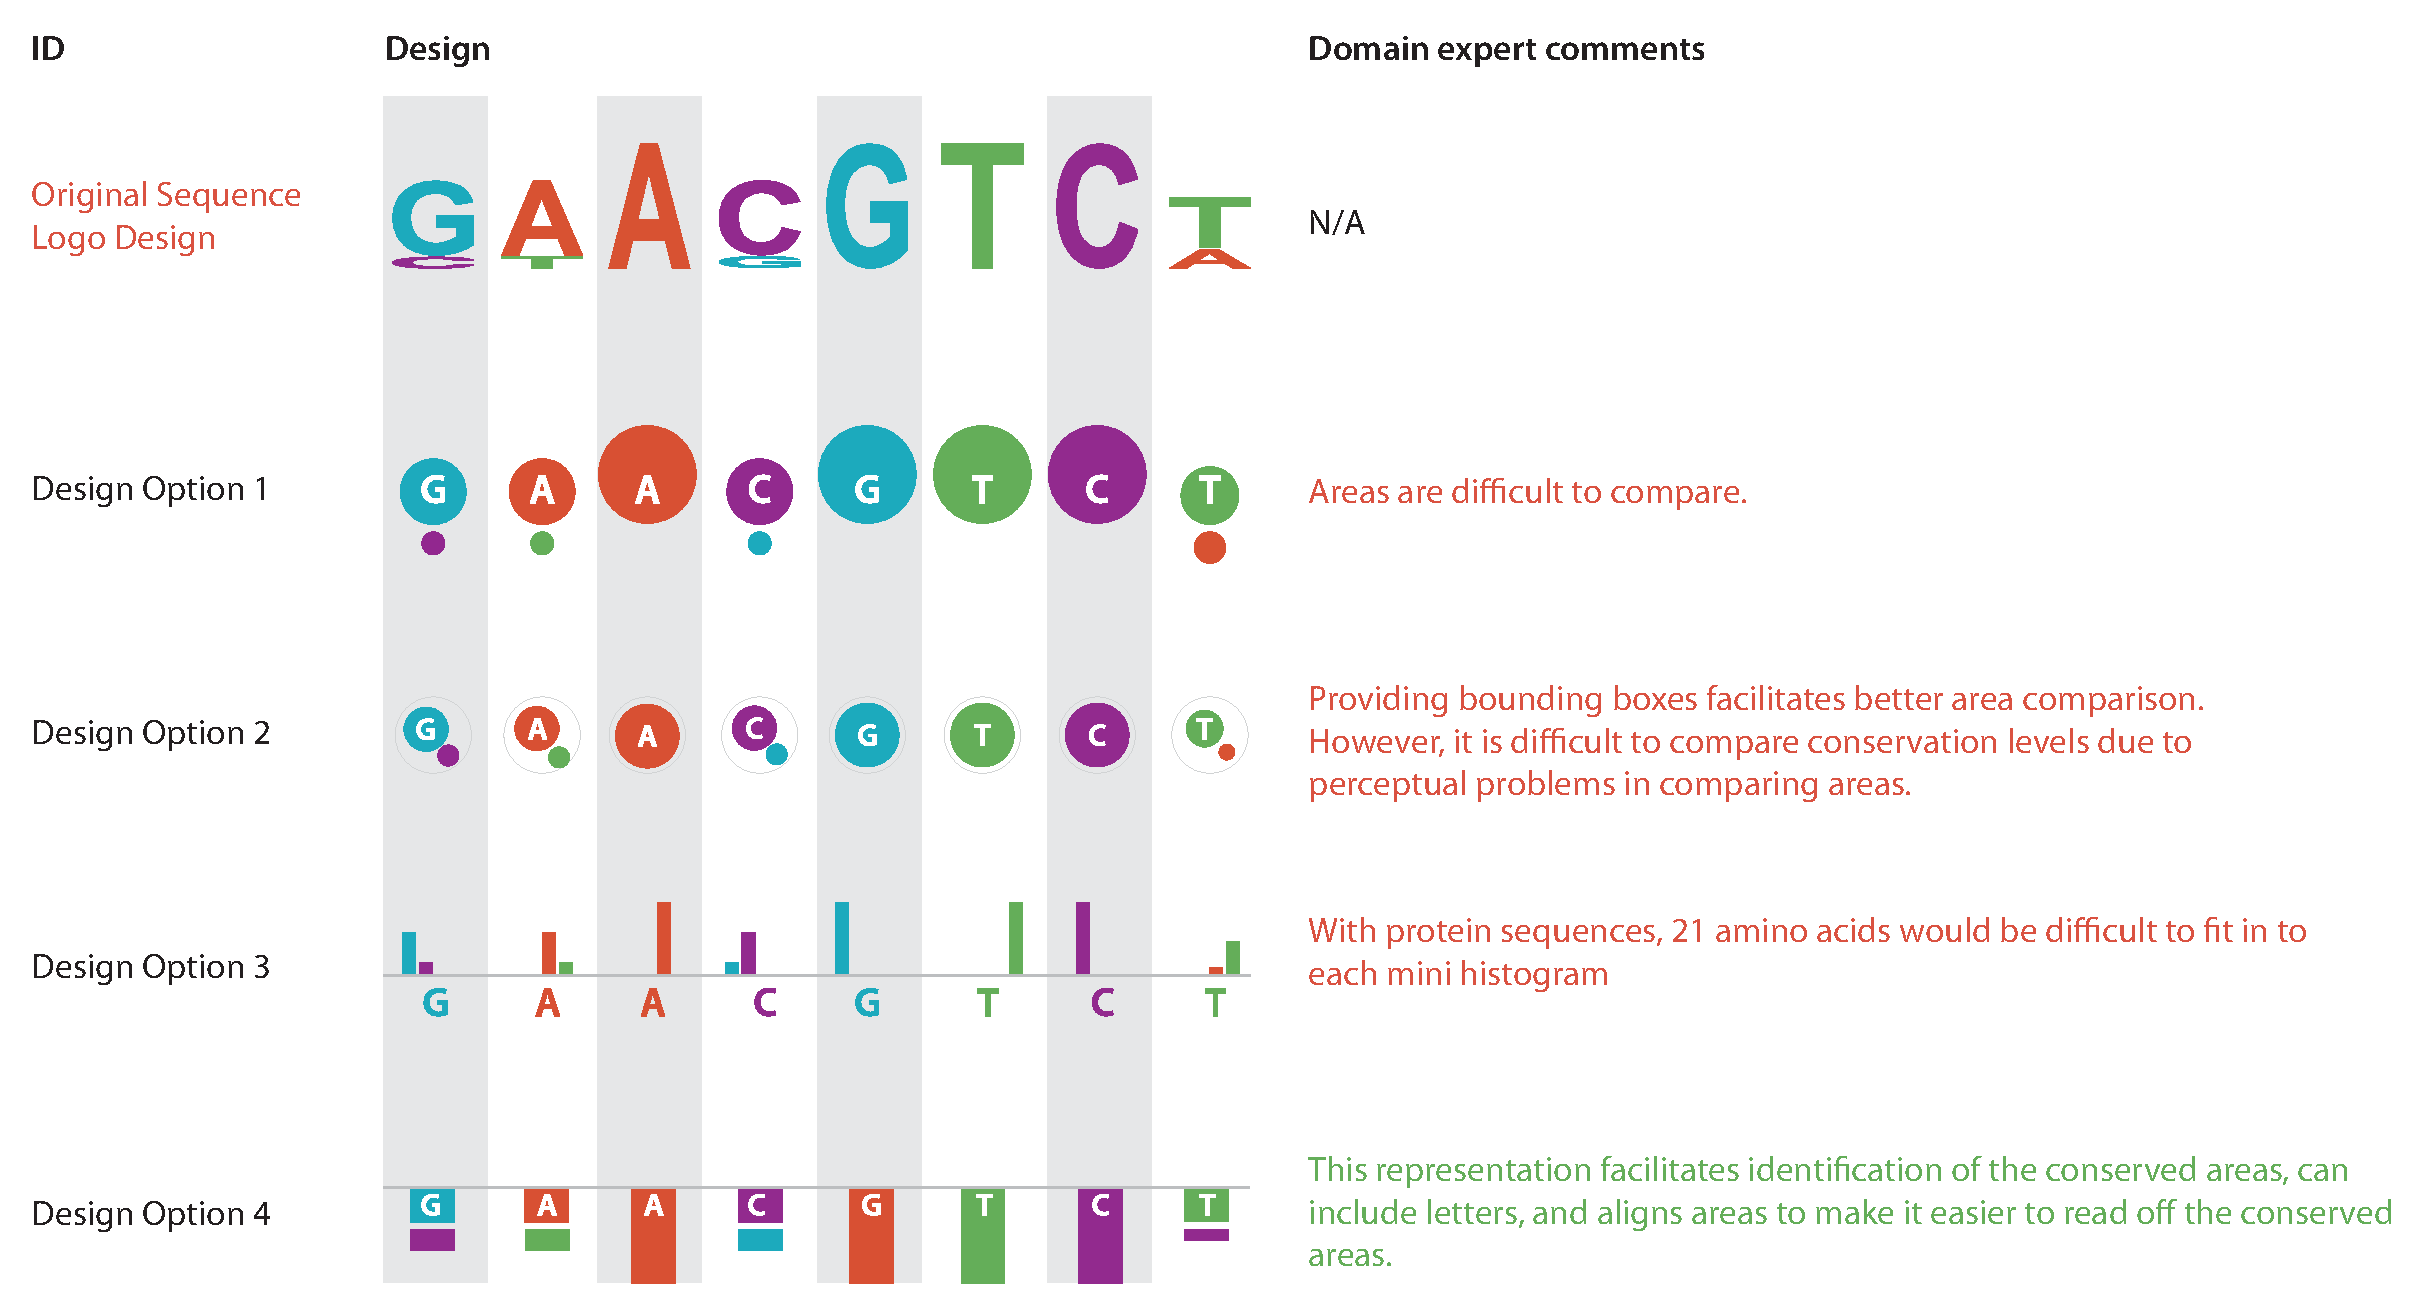
\includegraphics[width=\textwidth]{images/other_glyphs/sequence_logo/design_options}
\caption{A number of design options and reasons for excluding them based on research by Cleveland and McGill \cite{cleveland1984graphical} and Heer and Bostock \cite{heer2010crowdsourcing}.}
\label{fig:sequence_design_options}
\end{figure}

Our final design, shown in Figure \ref{fig:sequence-logo-design} uses filled bars to represent size in place of the letters.
The top `residues' (amino acids or nucleotides) are positioned at the top or bottom of the plot so that the conserved sequence can be read more easily than in the original logo.
The colours of the bars are a function of the type of amino acid.
However, these colours are not fixed and may be altered depending on how the user prefers to visually group residues.

\begin{figure}[b!]
\centering
\includegraphics[width=.75\textwidth]{images/other_glyphs/sequence_logo/sequence-logo-design}
\caption{Redesign of the sequence logo layout from the original (left) to the new version. Bars may be aligned to the top or bottom. At each position, residues are displayed in order of their conservation.}
\label{fig:sequence-logo-design}
\end{figure}

Amino acid residue side-chain charge and hydrophobicity strongly affect protein folding and its final 3D conformation, so any significant change in those qualities may result in a significant functional change.
By providing a visual aid to remind users of those dimensions, we offer the opportunity for enhanced interpretation.
Additionally, we experiment with another glyph-based approach, named ``Gestalt Lines'' \cite{brandes2013gestaltlines} to provide an additional indication of variance at a position. 

\begin{figure}[t!]
\centering
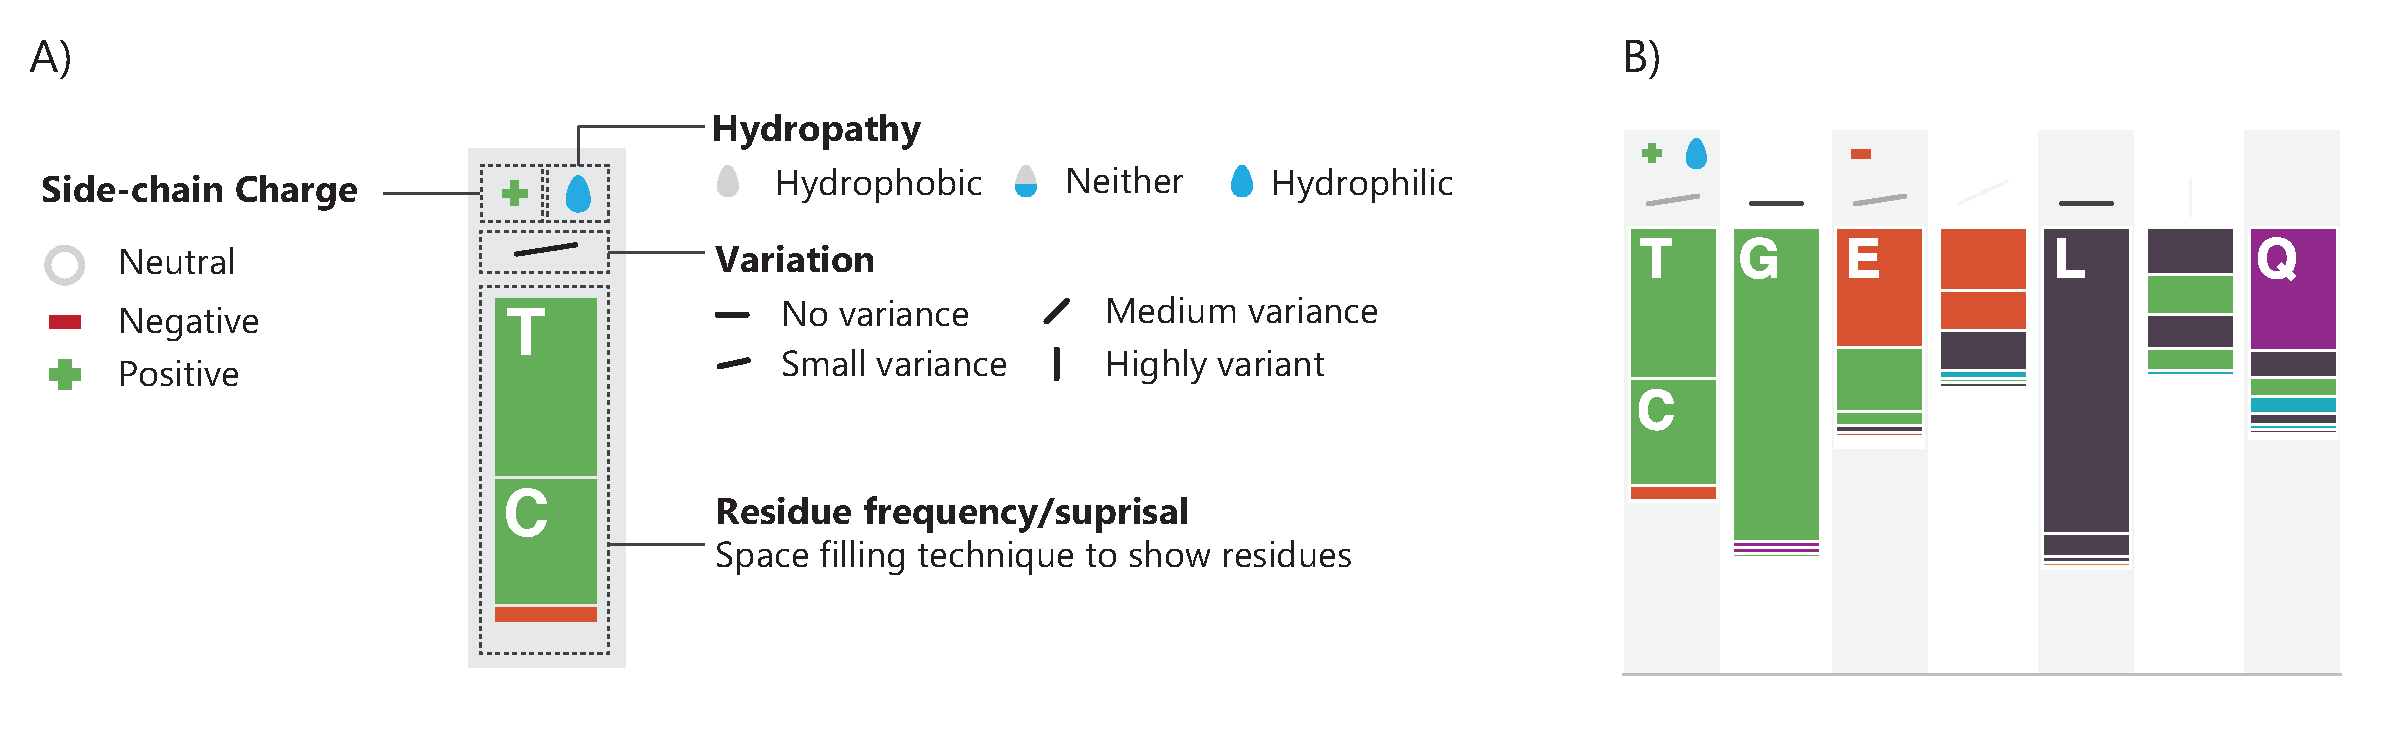
\includegraphics[width=\textwidth]{images/other_glyphs/sequence_logo/glyphs}
\caption{A) Overall glyph design has a number of regions to support glyph placement for interpretation, such as hydropathy, and side-chain charge.
Variation is also shown via ``GestaltLines'' \cite{brandes2013gestaltlines}.
B) A glyph is shown at a position in the sequence to form the overall sequence logo.}
\label{fig:glyphs}
\end{figure}

The glyphs provide an overall indication of any dominating characteristics of the amino acids present at a given position.
These glyphs, in context with the redesigned sequence logo are shown in Figure \ref{fig:glyphs}.
Glyphs for hydropathy and side-chain charge are only present in amino acid sequence logos. 

%-------------------------------------------------------------------------

\subsection{Evaluation}

\begin{figure}[b!]
\centering
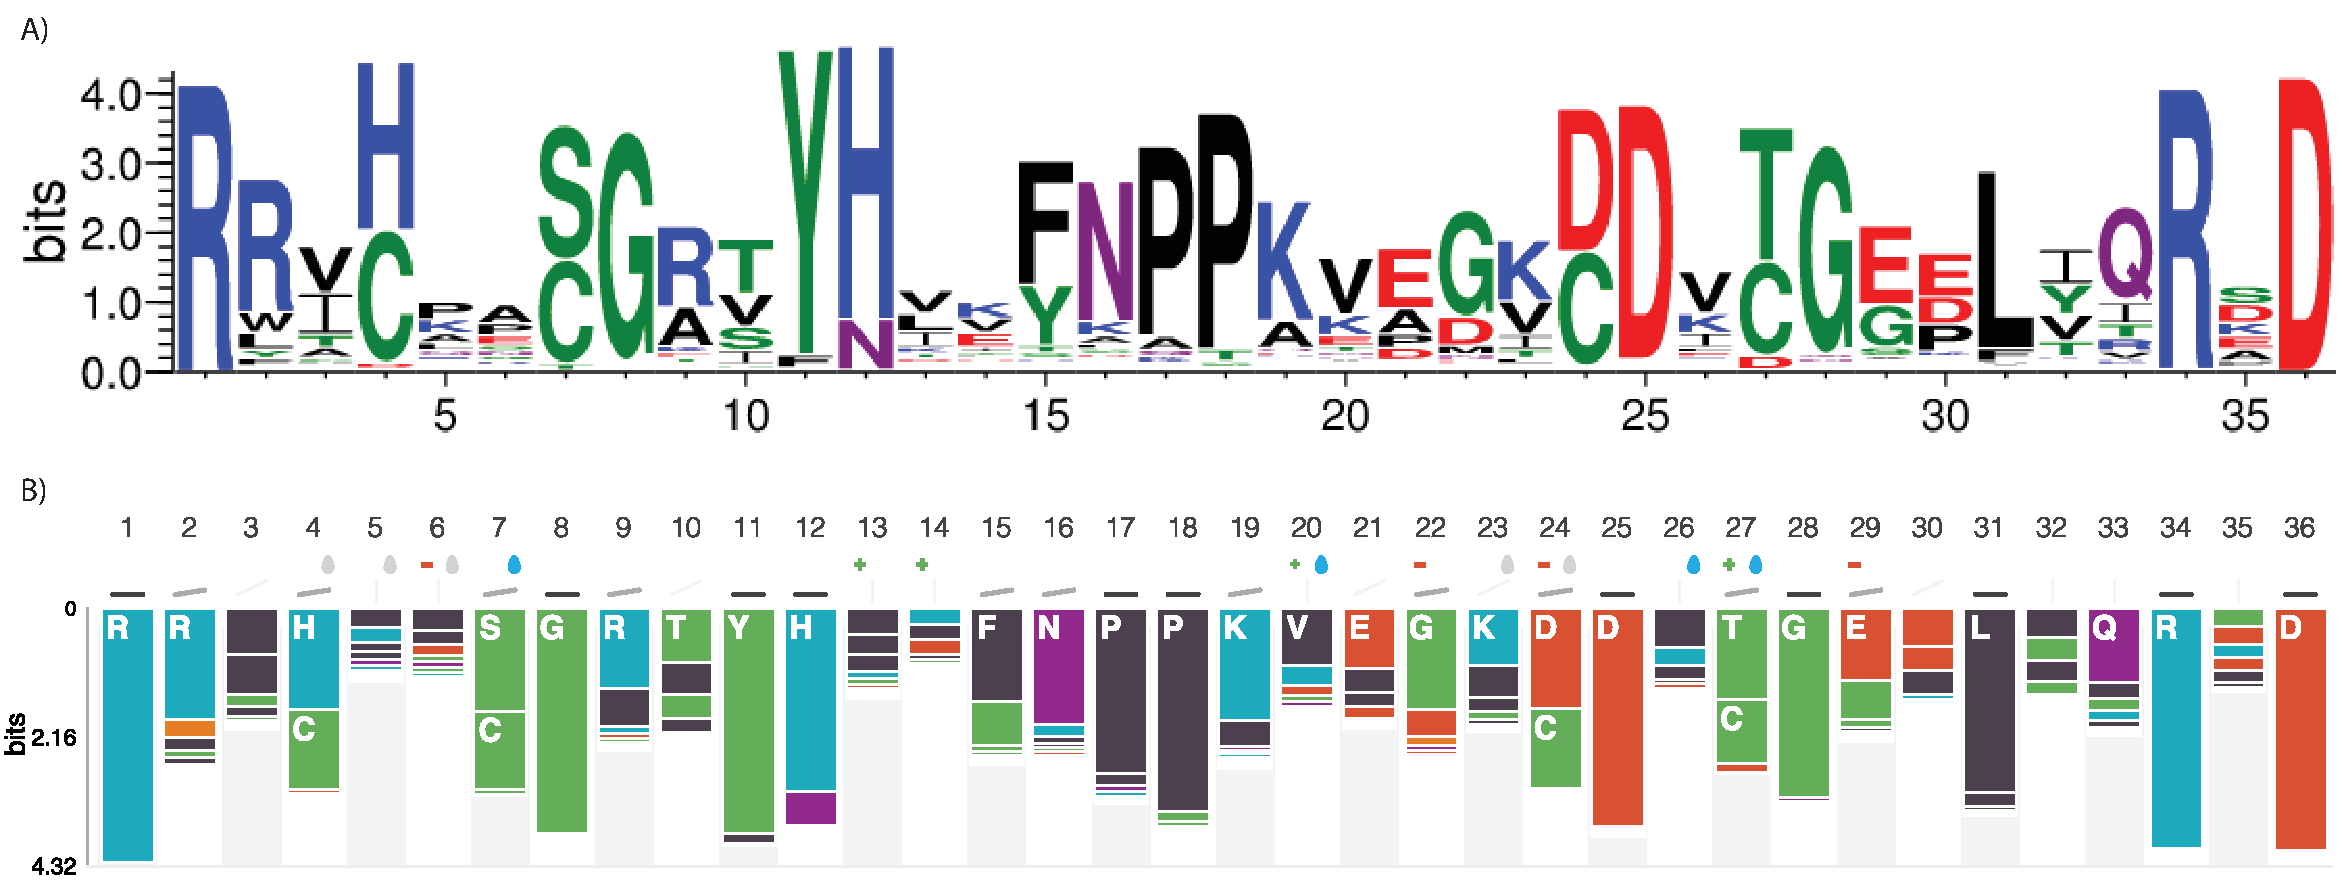
\includegraphics[width=\textwidth]{images/other_glyphs/sequence_logo/old_and_new_design}
\caption{A) Traditional sequence logo representation. B) New sequence logo representation.}
\label{fig:old_and_new}
\end{figure}

In order to assess if our changes helped biologists in their interpretation of sequence logos, we devised a survey focused on evaluating the ability to compare the size of letters in the old version of the sequence logo (see Figure \ref{fig:old_and_new} A) and the new version (Figure \ref{fig:old_and_new} B). We used the same data to create the two versions of the sequence logo and asked participants to determine which letter between two was the largest.
Our hypothesis, as stated earlier, is that it is harder to compare letters than blocks. Forty-one scientists (fifteen bioinformaticians, twenty-three biologists and three computer scientists) with varying levels of familiarity with sequence logos, took part in the survey.

\begin{figure}[t!]
\centering
\includegraphics[width=\textwidth]{images/other_glyphs/sequence_logo/evaluation}
\caption{Evaluation responses showing the ability to discriminate between conservation levels in the two designs of the sequence logo, old/original and new.}
\label{fig:evaluation}
\end{figure}

Figure \ref{fig:evaluation} shows survey results (upper part) and test images (lower part).
In three out of the four questions given to users, a higher number of correct answers were recorded with the new sequence logo.
The gain was significant for questions two and three, with up to twice as many correct answers with the new representation. The exception was in question four, where there was a small (8\%) advantage gained by using the original version.
The greater density of `G' over `L' may have lead to more people choosing correctly by chance, explaining the observation. More thorough experimentation would be needed to validate this hypothesis however.

The feedback from users regarding the glyphs was also largely positive with: 80\% of respondents agreeing that showing hydropathy was useful; 83\% agreeing that showing side-chain charge was useful; and 59\% indicating that the variance glyph using GestaltLines was useful.
The feedback led to the removal of the ``GestaltLines'' from the entropy-based height encoding since the level of variance can be adequately determined using bar height alone.
For frequency-based height encoding, ``GestaltLines'' are more useful since all bars are the same height.

The approval of our redesign was also measured with users asked to give their preference between Figures \ref{fig:sequence_logo_design_teaser} A and B. 95\% of respondents said that they preferred the new representation over the original, citing amongst others, `cleanliness' and `clarity' as major factors in their decision.
%
%\subsection{Contributions}
%We have presented a new design for the sequence logo that incorporates glyph-based techniques to aid interpretation. 
%We have also provided an implementation of this new logo available at \url{https://github.com/ISA-tools/SequenceLogoVis} that can be incorporated into the workflows of scientists for interactive use or inclusion in publications.
%Our usability tests showed that users generally found consensus sequence reading tasks easier with the new sequence logo. Users, on the whole, agreed that the new representation did a better job of improving the display of salient information.
%
%This work was published as a short paper and presented at EuroVis 2015 in a paper entitled \emph{Redesigning the Sequence Logo with Glyph-based Approaches to Aid Interpretation} \cite{CGF:maguire14-sp}.

